%%% The ``\documentclass'' command has one parameter, based on the kind of
%%% document you are preparing.
%%%
%%% [annual] - Technical paper accepted for presentation at the ACM SIGGRAPH 
%%%   or SIGGRAPH Asia annual conference.
%%% [sponsored] - Short or full-length technical paper accepted for 
%%%   presentation at an event sponsored by ACM SIGGRAPH
%%%   (but not the annual conference Technical Papers program).
%%% [abstract] - A one-page abstract of your accepted content
%%%   (Technical Sketches, Posters, Emerging Technologies, etc.). 
%%%   Content greater than one page in length should use the "[sponsored]"
%%%   parameter.
%%% [preprint] - A preprint version of your final content.
%%% [review] - A technical paper submitted for review. Includes line
%%%   numbers and anonymization of author and affiliation information.

\documentclass[annual]{acmsiggraph}

%%% If you are submitting your paper to one of our annual conferences - the 
%%% ACM SIGGRAPH conference held in North America, or the SIGGRAPH Asia 
%%% conference held in Southeast Asia - there are several commands you should 
%%% consider using in the preparation of your document.

%%% 1. ``\TOGonlineID''
%%% When you submit your paper for review, please use the ``\TOGonlineID''
%%% command to include the online ID value assigned to your paper by the
%%% submission management system. Replace '45678' with the value you were
%%% assigned.

\TOGonlineid{45678}

%%% 2. ``\TOGvolume'' and ``\TOGnumber''
%%% If you are preparing a preprint of your accepted paper, and your paper
%%% will be published in an issue of the ACM ``Transactions on Graphics''
%%% journal, replace the ``0'' values in the commands below with the correct
%%% volume and number values for that issue - you'll get them before your
%%% final paper is due.

\TOGvolume{0}
\TOGnumber{0}

%%% 3. ``TOGarticleDOI''
%%% The ``TOGarticleDOI'' command accepts the DOI information provided to you
%%% during production, and which makes up the URLs which identifies the ACM
%%% article page and direct PDF link in the ACM Digital Library.
%%% Replace ``1111111.2222222'' with the values you are given.

\TOGarticleDOI{1111111.2222222}

%%% 4. ``\TOGprojectURL'', ``\TOGvideoURL'', ``\TOGdataURL'', ``\TOGcodeURL''
%%% If you would like to include links to personal repositories for auxiliary
%%% material related your research contribution, you may use one or more of
%%% these commands to define an appropriate URL. The ``\TOGlinkslist'' command
%%% found just before the first section of your document will add hyperlinked
%%% icons to your document, in addition to hyperlinked icons which point to
%%% the ACM Digital Library article page and the ACM Digital Library-held PDF.

\TOGprojectURL{}
\TOGvideoURL{}
\TOGdataURL{}
\TOGcodeURL{}

%%% Replace ``PAPER TEMPLATE TITLE'' with the title of your paper or abstract.

\title{PerVERT: The Performance Visualization and Error Remediation Toolkit}

%%% The ``\author{}'' command takes the names and affiliations of each of the
%%% authors of your paper or abstract. The ``\thanks{}'' command takes the
%%% contact information for each author.
%%% For multiple authors, separate each author's information by the ``\and''
%%% command.

\author{Niels Joubert\thanks{e-mail:njoubert@cs.stanford.edu}\\ Stanford University %
\and Eric Schkufza\thanks{e-mail:eschkufz@cs.stanford.edu}\\ Stanford University}

%%% The ``pdfauthor'' command accepts the authors of the work,
%%% comma-delimited, and adds this information to the PDF metadata.

\pdfauthor{Niels Joubert, Eric Schkufza}

%%% Keywords that describe your work. The ``\keywordlist'' command will print
%%% them out.

\keywords{performance visualization, JIT, compiler, instrumentation}

%%% The ``\begin{document}'' command is the start of the document.

%%% If you have user-defined macros, you may include them here.

% example of a user-defined macro called ``remark.''
% \newcommand{\remark}[1]{\textcolor{red}{#1}}

\begin{document}

%%% A ``teaser'' image appears under the title and affiliation information,
%%% horizontally centered, and above the two columns of text. This is OPTIONAL.
%%% If you choose to have a ``teaser'' image, it needs to be placed between
%%% ``\begin{document}'' and ``\maketitle.''

\teaser{
   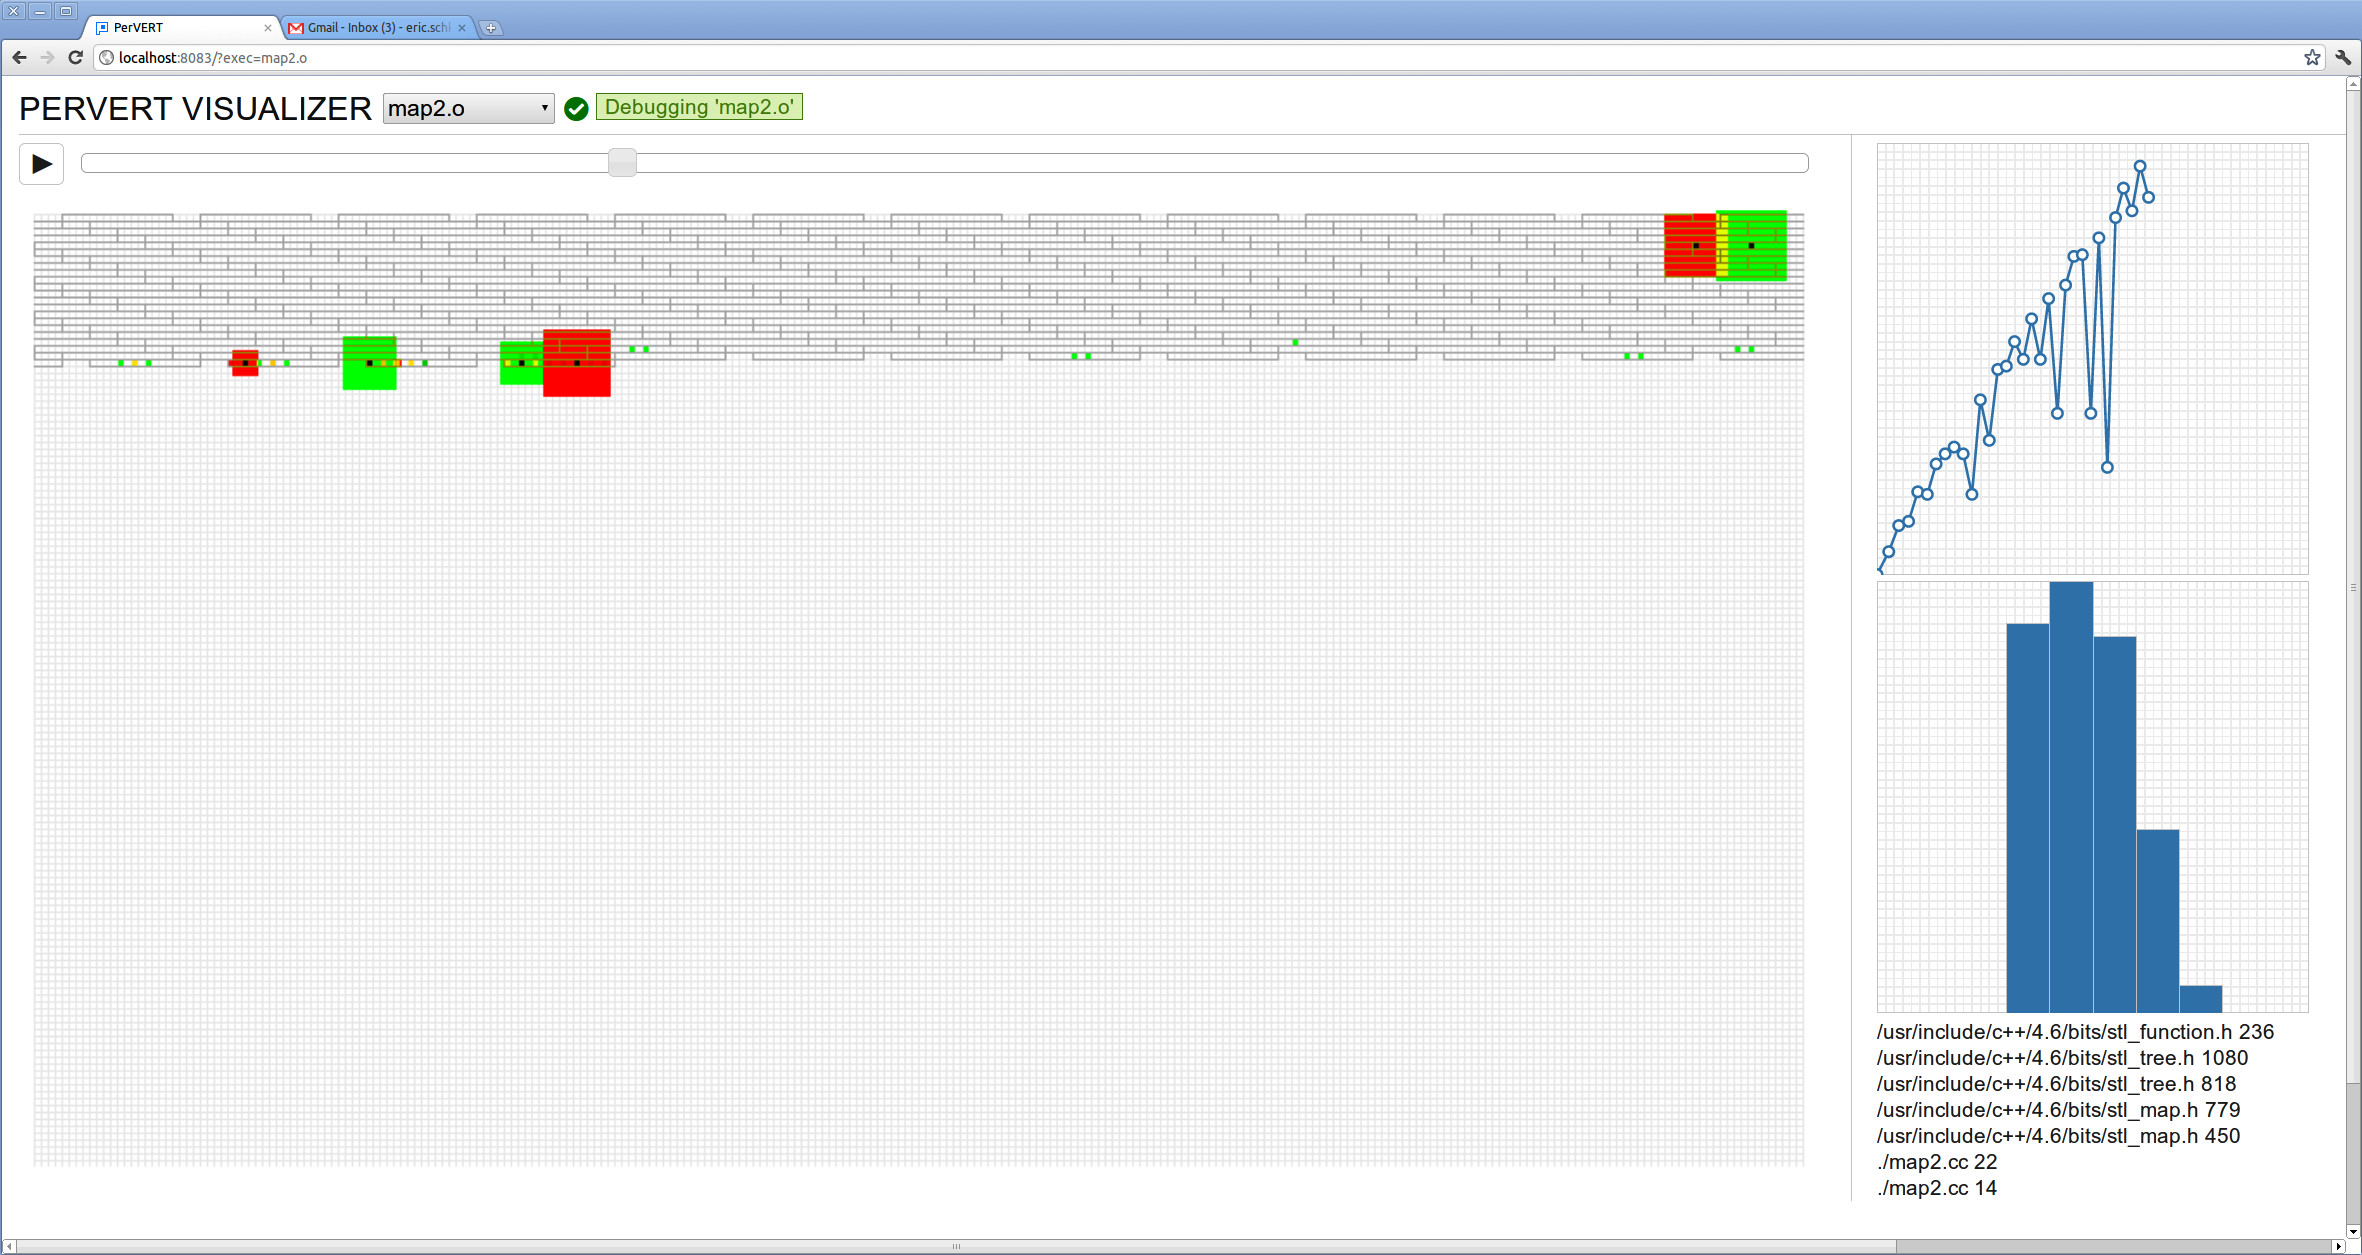
\includegraphics[height=3in]{images/pervert.png}
   \caption{Spring Training 2009, Peoria, AZ.}
}

%%% The ``\maketitle'' command must appear after ``\begin{document}'' and,
%%% if you have one, after the definition of your ``teaser'' image, and
%%% before the first ``\section'' command.

\maketitle

%%% Your paper's abstract goes in its own section.

\begin{abstract}

Performance tuning is an important step in the development large software systems. 
Examples include web-servers which routinely handle thousands of simultaneous content requests, 
  and petaflop supercomputers which perform physical simulations that span tens of thousands of cpu cores. 
As improvements in clock frequency slow and hardware trends continue towards increased parallelism, 
  the runtime performance of these and similar systems will become ever more a function of memory efficiency. 
Unfortunately, the ability to effectively reason about this phenomenon using existing tools such as valgrind, gprof, or gdb, 
  through a text-based interface, is limited, and tedious at best.

We present PerVERT, an instrumentation framework for logging a process's virtual memory traffic and a visualization suite for reasoning about common memory performance bugs: 
  Are memory accesses organized coherently in both spatial and temporal dimensions? 
  To what extent do these patterns differ based on program inputs or changes in source code?
\end{abstract}

%%% ACM Computing Review (CR) categories.
%%% See <http://www.acm.org/class/1998/> for details.
%%% The ``\CRcat'' command takes four arguments.

\begin{CRcatlist}
  \CRcat{I.3.7}{Computer Graphics}{Three-Dimensional Graphics and Realism}{Radiosity};
\end{CRcatlist}

%%% The ``\keywordlist'' command prints out the keywords.

\keywordlist

%%% The ``\TOGlinkslist'' command will insert hyperlinked icon(s) to your
%%% paper. This includes, at a minimum, hyperlinked icons to the ACM article
%%% page and the ACM Digital Library-held PDF. If you added URLs to
%%% ``\TOGprojectURL'' or the other, similar commands, they will be added to
%%% the list of icons.
%%% Note: this functionality only works for annual-conference papers.

\TOGlinkslist

%%% The ``\copyrightspace'' command 
%%% Do not remove this command.

\copyrightspace

%%% This is the first section of the body of your paper.

\section{Introduction}

  
  \begin{itemize}
  \item Many people care about having high performance codes, which need to be as fast as possible. 
  \item Performance means minimizing time -- interested in viewing events over time.
  \item Performance is often a function of memory efficiency because memory is so much slower than compute.
  \item Performance is considered a "black art" and very difficult to get right, since it's a secondary effect of code.

  \item Most debugging tools are built for correctness, which is a property of the computations done on the program's state. This leads to a control-flow-centric view of the world, where the transformations your code does is inspected.
  \item Performance is a more global property depending on the actual data usage, thus a data-centric view is a more natural fit.
  \item Performance is also a global property since data layout directly affects access patterns, which is state hidden from the code being written.
  \item Even simple code can cause incredibly complicated access patterns and consume lots of data.
  \item Thus, we want to use a visual approach to aggregate lots of data, and do this in a data-centric view that directly shows how memory is accessed.
  \end{itemize}
  
    The remainder of this paper is structured as follows:

    Design Goals - how we want to build this system
    Design - the visualizations we build to support this system
    Implementation - how we built the system
    Related Work
    Future Work 
    Conclusion
  
\section{Design Goals}

  \subsection{Binary Instrumentation}
  \begin{itemize}
  \item At what level do we work? Performance depends on everything happening in your program, including the parts you have no insight into - libraries and system calls/
  \item It lowers the barrier to performance tuning when the same toolset can inform you about your code and the libraries you are using.
  \item Workin at a binary level provides transparency through everything an app uses, including system and third party libs.
  \end{itemize}

  \subsection{Remote Analysis}
  \begin{itemize}
    \item development vs production machines look very different
    \item often need to perftune remotely
    \item ideal to ship as little data from back-end to front-end, so analysis runs on back-end and vis runs on front-end.
  \end{itemize}

  \subsection{On-Demand Analysis}
  \begin{itemize}
    \item massive amounts of data, aggregated into many different ways, with multiple views of this data
    \item cannot do all analysis ahead of time
    \item do no want to do unneeded analysis
    \item thus we build a tool that can do analysis on-the-gly
  \end{itemize}
  

\section {Design}
  \subsection{Memory Map}
    \begin{itemize}
      \item PICTURE OF MEMMAP
      \item Performance is a global property 
      \item Therefore: Grid-based representation of the virtual address space.
      \item Physical cache structure has a huge impact on performance -- represented directly in the visualization.    
      \item Therefore: Rows correspond to cache lines.
      \item Memory events happen over time: Visualize as animation
      \item One memory location can be used for many different malloc'd regions, therefore not a static snapshot over all time
      \item Four types of events: mallocs, frees, reads, writes
      \item Visual cues for malloced regions - heavy outlines for those cells
      \item Visual cues for reads and writes - highlight memory accesses by coloring cells.
      \item Visual history of recent accesses - s
      \item Fireworks to highlight local changes.
      \item Alpha blending gives cues to access patterns: R, W, mix
   \end{itemize}

Interaction:
   \begin{itemize}   
      \item Watching the animation shows visual queues leads to interesting events being very obvious, begs further inspection.
      \item Pausing, Stepping fwd and back allows deeper inspection of interaction between temporally local events.
      \item Scrubbing and Jumping through all time quickly allows for quick memory access comparisons at different points in time.
      \item This implementation of the memory map aids in identifying problem areas.
    \end{itemize}
  
  \subsection{Code Context}
    %\begin{itemize}
    %  \item PICTURE OF CODE CONTEXT
    %  \item Every event was caused by an instruction, and thus has an associated context: the stacktrace that caused it.
    %  \item We wish to find the code that caused this event.
    %  \item We display entire stacktrace, incl. user and library code
    %\end{itemize}

    Every event in a memory trace is caused by a single instruction with an associated context: the stacktrace which produced it.
    This information is extremely valuable.
    It allows the user to associate behavior in the memory map visualization (both good and bad) 
      with the source code that produced it.
    Accordingly, we display stack traces for every frame in the memory map visualization, 
      including both user code and library code.
  
  \subsection{Context Access Patterns}
    \begin{itemize}
      \item PICTURE OF TWO ACCESS PATTERNS
      \item Once a piece of code is identified, the user can further inspect the behavior of this context.
      \item For a given context we can drill down into the memory access patterns it causes
      \item It's common to reason about the stride of a context - understanding the distances between accesses it causes.
      \item Hitogramming strides gives insight into the caching behaviour of this code.
      \item We also want to distinguish whether a context is always problematic or only in this instance, histograms does not show time.
      \item A complementary view to show access pattern of context over all time
      \item Inspecting a combination of these two views gives an overall insight into the caching behavior of the code and suggests approaches to fix it - change the stride or change the data layout.
    \end{itemize}

\section {Implementation}
  %\begin{itemize}
  %  \item SYSTEM DIAGRAM
  %  \item Built up from three parts -- described below
  %\end{itemize}

	\begin{figure}[t]
		\centering
    SYSTEM DIAGRAM
    %\includegraphics[scale=0.55]{figures/isa.pdf}
		\caption{The implementation of PerVERT.}
    \label{fig:system}
	\end{figure}

  PerVERT consists of five separate components as suggested by Figure \ref{fig:system}:
    a binary instrumentation tool for recording memory traces from program executions,
    an analysis engine for indexing those traces,
    a backend data server for performing on demand analyses on top of those indices,
    an HTTP JSON server for serving that data,
    and a front end for visualizing that data to the user.
  These components are described in detail below.  

  \subsection{Binary Instrumentation}
%    \begin{itemize}
%      \item What it is: Pintool plugin
%      \item Programming language agnostic instrumentation tool.
%      \item Works on code written in any language that compiles to x86 binary.
%      \item Produces memory trace
%      \item Intercept X86 to find read/write instructions
%      \item Intercept function calls to find malloc/free
%      \item Save as trace file
%    \end{itemize}

    The binary instrumentation component of the PerVERT pipeline is a plugin for Intel's pintool \cite{Luk:2005:PBC:1065010.1065034}:
      a language agnostic JIT instrumentation framework for X86 object files.
    Because of this, PerVERT can be run object code irrespective of its original source language.

    PerVERT produces a memory trace by intercepting each of a program's instructions, just before they are executed.
    Reads and writes are found by extracting the arguments from opcodes which are known to touch memory,
      wheras calls to malloc and free are found by identifying jumps to addresses which correspond to those functions
      in the symbol table.
    Reads and writes to addresses that do not appear within malloc'ed regions of the heap are ignored.  
    The resulting trace is written out to a file, and each element is annotated with the stack context in which it occurred.  

  \subsection{Backend}
    %\begin{itemize}
    %  \item System is designed to handle massive amounts of data.
    %  \item Static index built over that data.
    %  \item On demand analysis done in response to user interaction.
    %  \item To optimize this, we unify analysis of and interface to data.
    %\end{itemize}

    The PerVERT backend is designed to handle massive amounts of data.
    It is no uncommon for even a modestly sized program to generate in excess of one million memory events.
    The PerVERT backend builds a static index over each memory trace that it produces, 
      and performs on demand analysis when necessary in response to user interactions.
    To minimize the amount of time spent transmitting the resulting data, 
      PerVERT's analysis engine and data server are unified.
    We describe this architecture below.

    \subsubsection{Index}
      %\begin{itemize}
      %  \item What is is: Persistent long running analysis server
      %  \item Read and index trace files (what indices?)
      %  \item Read and index debug symbols from executable (what symbols?)
      %\end{itemize}

      The PerVERT analysis engine is responsible for building static indices over memory traces.
      This includes tracking memory events by type: read, write, malloc, or free,
        as well as by context.
      For any event, the analysis engine records the stack context that produced the event, 
        as well as pointers to all other events produced by that context.       
      The PerVERT analysis engine also indexes a program's debugging symbol library so that it can decode
        hexademical stack traces to lists of file-line pairs.

      % june sandwich -- 
      % niels below

    \subsubsection{Server}
      \begin{itemize}
        \item HTTP JSON server
        \item Serves frontend / presents JSON api
        \item Persistently captures all executables so that you can do comparisons between runs.
        \item A stateless api so that multiple users can view the same data or one user can close and come back.
      \end{itemize}

  \subsection{Frontend}
    \begin{itemize}
      \item Web app: user interaction initiates asynchronous request for textual data - then render as visualizations.
      \item Caching layer stores interaction history to minimize backend communication
      \item Use canvas to draw memory space / pixel pushing.
      \item D3 to draw aggregate statistics
    \end{itemize}

\section {Example Applications}
  % No outline - we never specced this paragraph out

  \subsection{Algorithm}
    To evaluate PerVERT, we built a test suite of algorithmic variants for a same simple routine
      which one would expect to find a scientific computation kernel.
    (1) Create a container of objects on the heap.
    (2) Write values to each of those objects.
    (3) Read values from each of those objects.
    (4) Free the objects and the container.

    The variants differ only in the type of container used.

  \subsection{Variants}
    \begin{itemize}
      \item C++ array WITH STREAMING THROUGH
      \item C++ STL vector WITH PICTURE OF GROWTH AND REALLOC
      \item C++ STL map WITH PICTURE OF BINARY SEARCH
      \item Haskell list WITH PICTURE
    \end{itemize}

\section{Related Work}

Visualizing Memory Graphs\cite{zimmerman:2001:VMG}, made the same observation that you want to drill down into memory structures, but they took a very different approach: they care about structures being built rather than than access to these structures. While we find this to be a useful inspection for debugging purposes, it does not directly show performance. It's a great example of memory visualization for debugging rather than performance.

KCacheGrind allows you to visualize the static structure of your code - similar to our stack traces - and also attaches performance events to it. While we take a very visual approach to this, KCacheGrind bubbles up statistics directly related to cache performance. This is useful for identifying issues, but we claim that our approach gives a direct visualization of the reasons behind the cache performance.

\section{Future Work}
  \subsection{Visualization and Interaction}
  \begin{itemize}
    \item Diffmaps for comparing across revisions
    \item Aggregate views for massive amounts of data
    \item User-defined data filtering
    \item Bookmarking, Auto-Bookmarking
  \end{itemize}

  \subsection{Data Collection and Analysis}
  \begin{itemize}
    \item Physical memory simulator
    \item Supporting incomplete data / sampling
    \item Selective data capture
  \end{itemize}

\section{Conclusion}
  Do this last.

\bibliographystyle{acmsiggraph}
\bibliography{template}
\end{document}
